% Chapter 3

\chapter{\uppercase{Implementation of the Project}} % Main chaptble to logier title
\label{ch:chap3} % For referencing
On launching the application, the user will be able to register by providing their details and user token provided by their distributor. With this, the user will be able to login and specify their requirements. They can update this regularly. The user will be prompted to enter their address and with the help of  google maps API, he/she will be able to point to their accurate location. 







%\section{\uppercase{View of Tables}}
%Sample view  is shown in Table \ref{tab:first} and an example is given in Table~\ref{tab:second}.


\section{\uppercase{Application Screenshots}}
%Examples of pictures are shown in Figure \ref{fig:one} and Figure \ref{fig:two}.
\begin{figure}[h]
\begin{center}
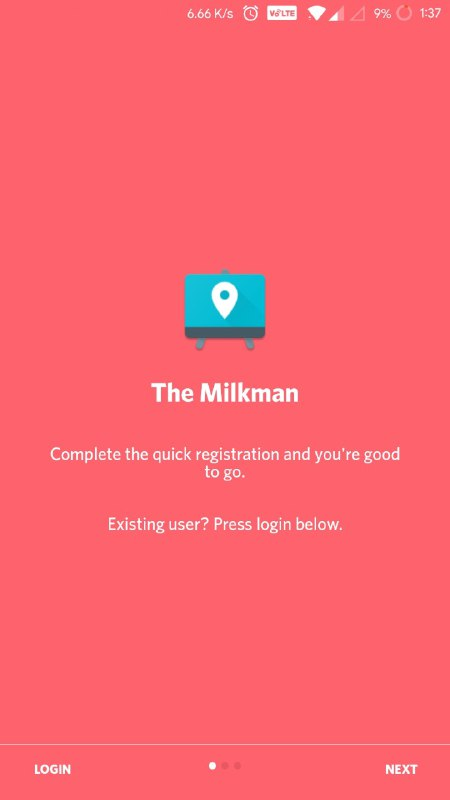
\includegraphics[scale=0.6]{3/one.jpeg}
\caption{Home page}
\label{fig:one}
\end{center}
\end{figure}

\begin{figure}[h]
\begin{center}
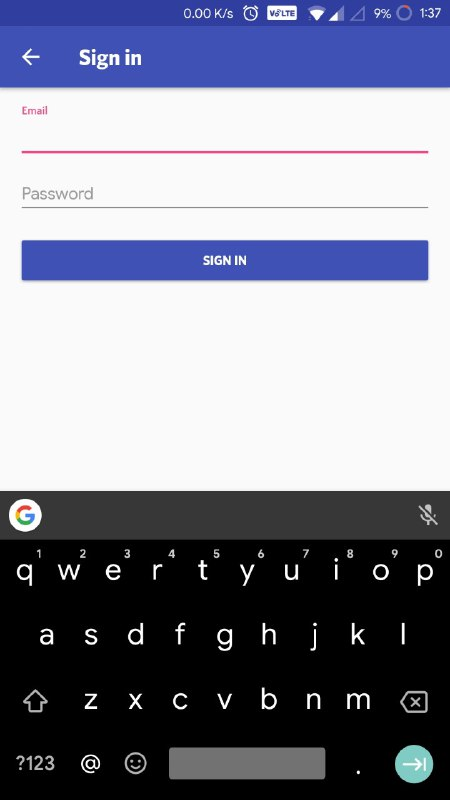
\includegraphics[scale=0.6]{3/two.jpeg}
\caption{Sign in!}
\label{fig:two}
\end{center}
\end{figure}

\begin{figure}[h]
  \begin{center}
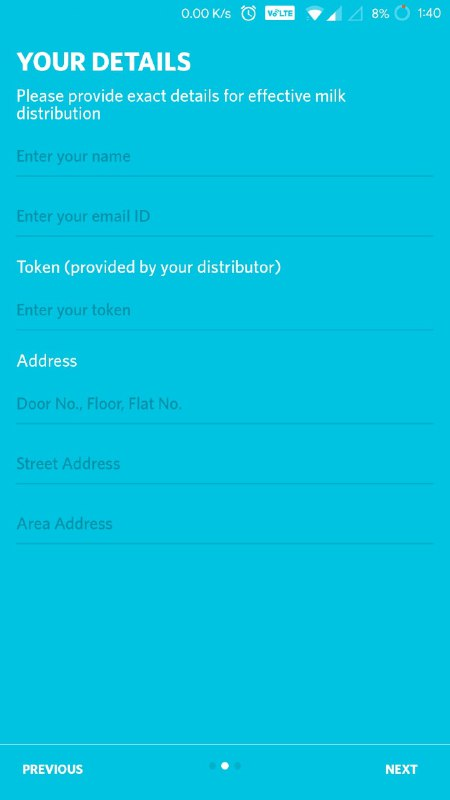
\includegraphics[scale=0.6]{3/three.jpeg}
\caption{Registration}
\label{fig:two}
\end{center}
\end{figure}

\begin{figure}[h]
  \begin{center}
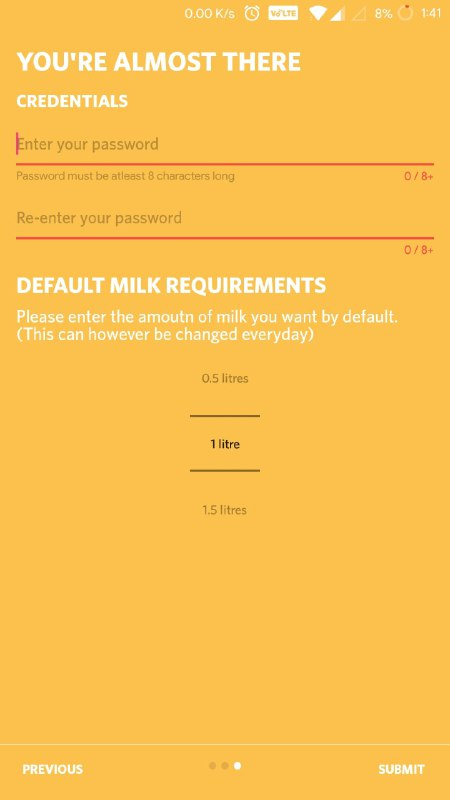
\includegraphics[scale=0.6]{3/four.jpeg}
\caption{Login and requirements}
\label{fig:two}
\end{center}
\end{figure}

\begin{figure}[h]
  \begin{center}
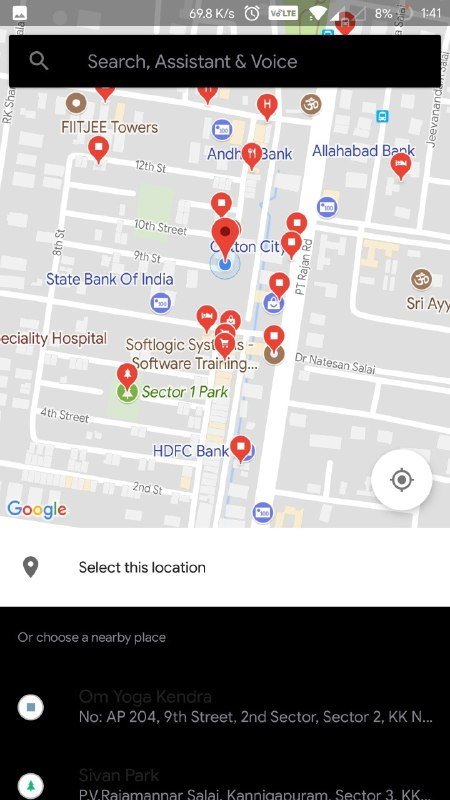
\includegraphics[scale=0.6]{3/five.jpeg}
\caption{Users latitue and longitude}
\label{fig:two}
\end{center}
\end{figure}

\begin{figure}[h]
  \begin{center}
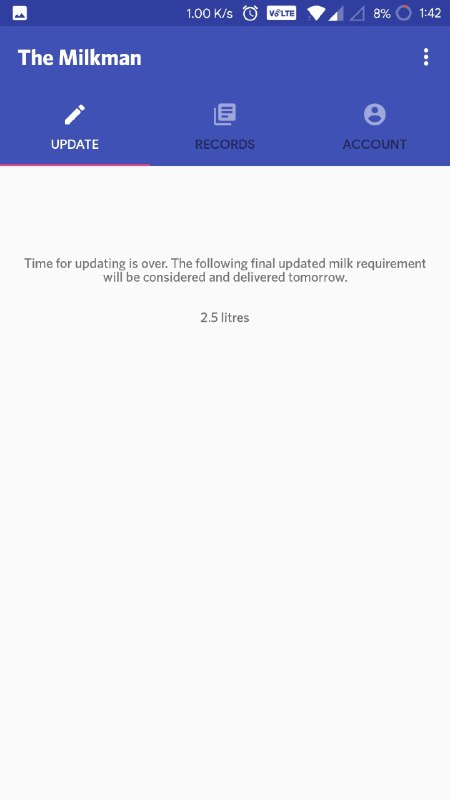
\includegraphics[scale=0.6]{3/six.jpeg}
\caption{Dashboard}
\label{fig:two}
\end{center}
\end{figure}

\begin{figure}[h]
  \begin{center}
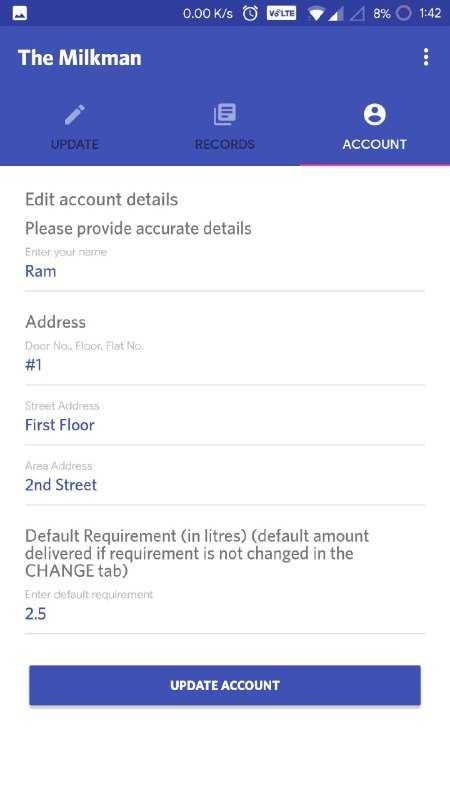
\includegraphics[scale=0.6]{3/seven.jpeg}
\caption{User details}
\label{fig:two}
\end{center}
\end{figure}

\begin{figure}[h]
  \begin{center}
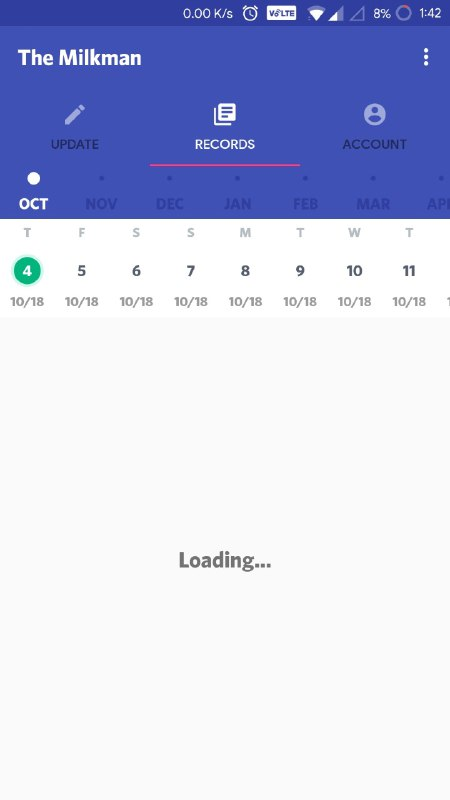
\includegraphics[scale=0.6]{3/eight.jpeg}
\caption{Consumption History}
\label{fig:two}
\end{center}
\end{figure}

\begin{figure}[h]
  \begin{center}
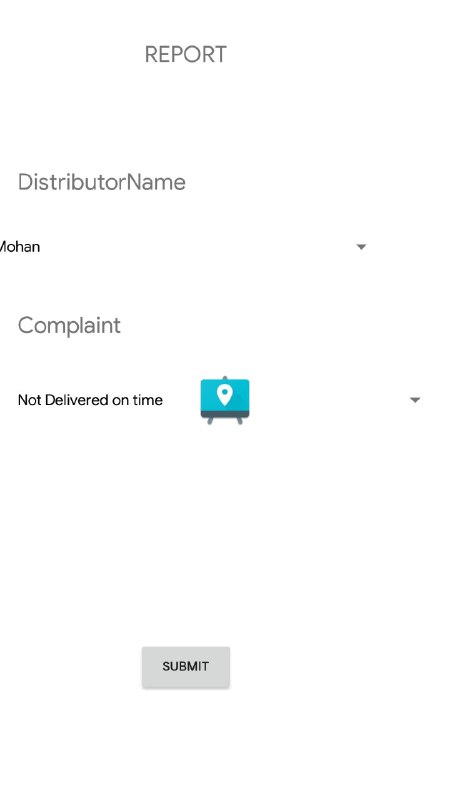
\includegraphics[scale=0.6]{3/nine.jpeg}
\caption{Complaints}
\label{fig:two}
\end{center}
\end{figure}

\begin{figure}[h]
  \begin{center}
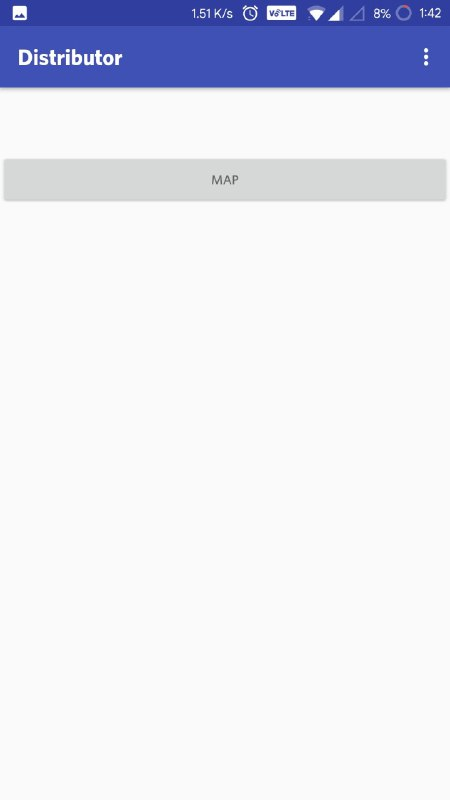
\includegraphics[scale=0.6]{3/ten.jpeg}
\caption{Distributor's interface}
\label{fig:two}
\end{center}
\end{figure}

\begin{figure}[h]
  \begin{center}
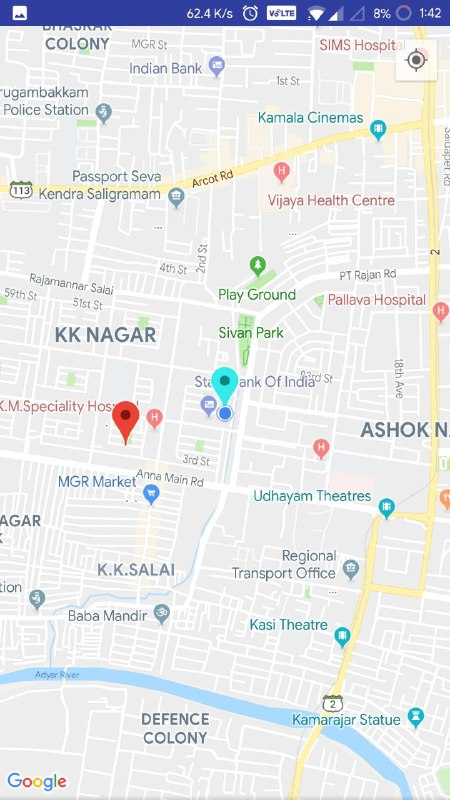
\includegraphics[scale=0.6]{3/eleven.jpeg}
\caption{Delivery}
\label{fig:two}
\end{center}
\end{figure}

\begin{figure}[h]
  \begin{center}
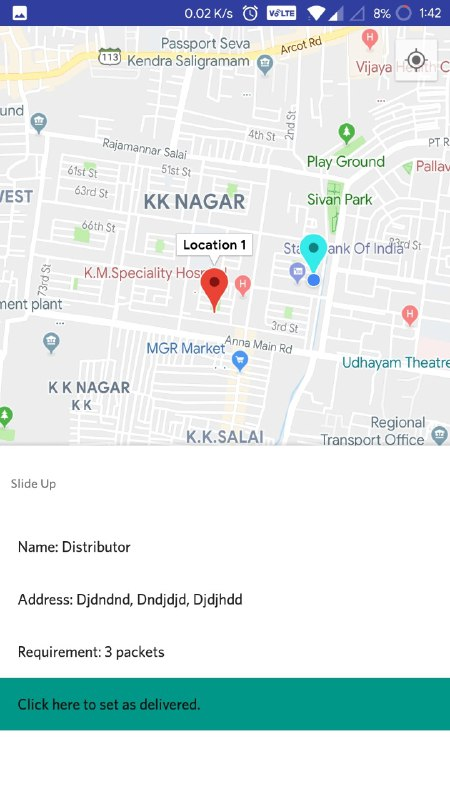
\includegraphics[scale=0.6]{3/twelve.jpeg}
\caption{Delivery }
\label{fig:two}
\end{center}
\end{figure}

\begin{figure}[h]
  \begin{center}
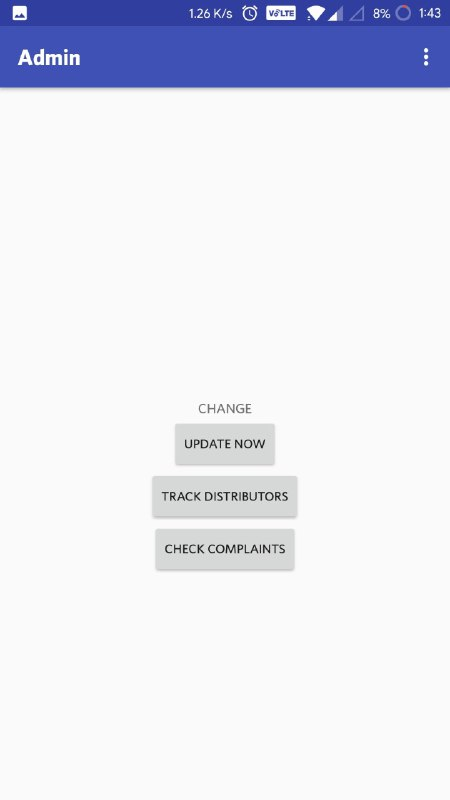
\includegraphics[scale=0.6]{3/thirteen.jpeg}
\caption{Admin Interface}
\label{fig:two}
\end{center}
\end{figure}

\begin{figure}[h]
  \begin{center}
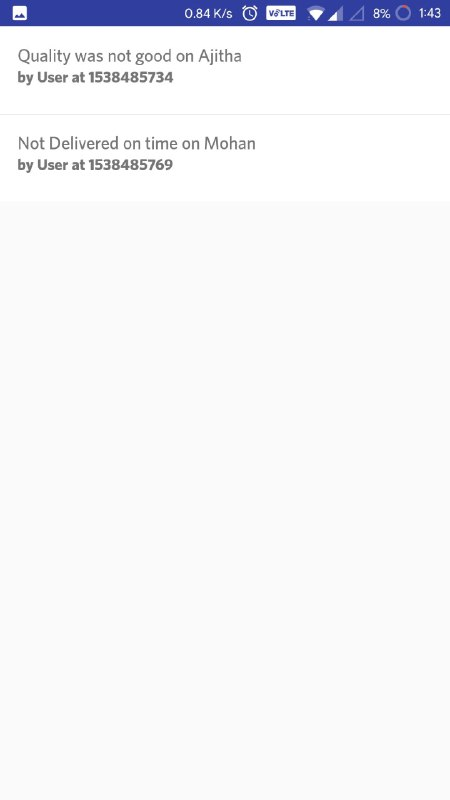
\includegraphics[scale=0.6]{3/fourteen.jpeg}
\caption{Displaying Complaints}
\label{fig:two}
\end{center}
\end{figure}







